% !TeX root = RJwrapper.tex
\title{Comparing Multiple Survival Functions with Crossing Hazards in R}
\author{by Hsin-wen Chang, Pei-Yuan Tsai, Jen-Tse Kao and Guo-You Lan}

\maketitle

\abstract{
It is frequently of interest in time-to-event analysis to compare multiple survival functions nonparametrically. %Existing R packages all utilize log-rank-type tests for the task. 
However, when the hazard functions cross, tests in existing R packages do not perform well. 
To address the issue, we introduce the package \pkg{survELtest}, which provides tests for comparing multiple survival functions with possibly crossing hazards. 
Due to its powerful likelihood ratio formulation, this is the only R package to date that works when the hazard functions cross.
%20190219 The tests are based on nonparametric likelihood ratio statistics that are known to produce tests with optimal power.
%20190219 Further, the statistics avoid the pitfall of the log-rank-type formulation, in which negative and positive differences between the estimated hazard functions cancel with each other in a weighted sum.
%We briefly describe and contrast the methods used in  \pkg{survELtest} and existing R packages. 
%In applications to data from randomized clinical trials and simulated datasets, w
We %provide code examples to
illustrate the use of the procedures in  \pkg{survELtest} by applying them to data from randomized clinical trials and simulated datasets. We show that these methods lead to more significant results than those obtained by existing R packages.
% and compare their performances. %with existing R packages.
%We show they can better detect differences among the survival functions when the hazard functions cross. %, compared with the log-rank-type tests.
}

\section{Introduction} %setup
The nonparametric comparison of multiple survival functions is of interest in numerous biomedical settings, such as clinical trials \citep{Retal:2015}, preclinical studies \citep{Letal:2015} and observational studies \citep{Letal:2013} with right-censored time-to-event endpoints.  It has been implemented in existing R packages using log-rank-type statistics. However, these log-rank-type tests
%While there have been \proglang{R} packages available for the task, 
% 20190106
%they 
can fail to detect differences among survival curves when the hazard functions cross.
%Specifically, they can fail to detect a difference among the survival curves, even when the estimated survival functions (called Kaplan--Meier curves) suggest otherwise. i
For example, consider the Kaplan--Meier (KM) estimated survival functions in Figure \ref{fig:hepatitis} for the treatment and control groups of patients in a randomized clinical trial. There is a clear gap between the survival curves, which we would expect to be detected by a reasonable statistical test. Nevertheless, the log-rank test provided in the \CRANpkg{survival} \cite[][]{survival:2018} package returns a $p$-value of $0.07$, indicating no significant difference between the two survival functions at $\alpha=0.05$. 
%based on right-censored data
%Note that in this case the gap between the survival curves shrinks in the middle of the follow-up period, suggesting that the estimated hazard functions may cross at some time point. % in this period.
%20200114
Note that in this case the gap between the survival curves shrinks then widens in the middle of the follow-up period, suggesting that the estimated hazard functions may cross at some time point.


\begin{figure}[H]
	\centerline{\includegraphics[width=0.5\columnwidth]{figures/paper_survELTest_hep_surv_20191220.pdf}} %,totalheight=2.0in
	\caption{Estimated survival functions for treatment (solid line) versus control (dashed line) groups, based on a randomized clinical trial for treatment of severe alcoholic hepatitis \citep[][]{hepatitis:2011}.}
	\label{fig:hepatitis}
\end{figure}

% 20190106
% first talk about haz, then while there have been? --- see intro_switch...
% focus on interpretation of survival functions
The need to compare survival functions with crossing hazards has been documented in the statistics literature \citep[see, e.g.,][]{PF:1989, YP:2010}. 
% to-polish
%The difference between hazard functions reflect instantaneous treatment effect, whereas the difference between survival functions embodied cumulative treatment effect. 
%This is an important issue becuase t
There are many practical situations in which the hazard functions cross, indicating that the instantaneous treatment effect changes direction.
For example, some treatments are initially harmful due to toxicity or other complications, but may be beneficial later on. Other treatments can have short-term benefits but produce side effects in the long run.
Despite the varying instantaneous treatment effect, the cumulative treatment effect can still be positive, as reflected by a positive difference between the treatment and control survival functions throughout the follow-up period. It is important to be able to detect such a difference, as the treatment would be worth considering in this case. %as long as the cumulative treatment effect is postivie.
To this end, an adaptive weighted log-rank test was implemented in  the R  package \CRANpkg{YPmodel} \citep[][]{YPmodel:2015}, but this test involves a parametric assumption on the hazard functions, is limited to two-sample comparisons, and cannot deal with the general $k$-sample situation.
Another method, the restricted mean survival time (RMST) approach,  was implemented in  the R  package \CRANpkg{survRM2} \citep[][]{survRM2:2017}. However, to our knowledge the RMST method can only deal with two-sample comparisons nonparametrically. For the $k$-sample case, certain model-based assumptions still need to be made \citep[see, e.g.,][]{CTU:2016}.

%The issue that have are gaining attention in recent years \added[id=hc]{more on this?}. 
% Q: Do we need to say the importance of crossing hazards function??

% what we do and improve, in terms of the estimated haz... (better than introducing more about log-rank anyway)
% directly compare not clear... 'in formulation' etc may be better...
To address this issue, % polish later
the package \CRANpkg{survELtest} \cite[][]{survELtest:2020} provides nonparametric tests that can deal with general $k$-sample comparisons while accounting for possibly crossing hazards. It avoids the pitfalls of log-rank-type statistics, in which negative and positive differences among the estimated hazard functions cancel each other in a weighted sum (see Section \nameref{sec:lit_tests} for more details). Further, the statistics are constructed using empirical likelihood (EL),
which has been shown to produce tests with optimal power \citep[see, e.g.,][]{K:2012}. %at each time $t_i$.
%introduce EL
EL is a nonparametric likelihood which does not assume that the data come from %without the need to assume 
a particular parametric family of distributions. It serves as the basis for constructing a nonparametric likelihood ratio (i.e., the EL ratio), which leads to more efficient inference than
%The benefit of using a likelihood ratio test is to gain power over 
Wald-type procedures such as log-rank-type tests, %that are based on a difference between the estimated parameters of interest, 
as seen in the literature on parametric \citep[see, e.g.,][]{M:1994} and nonparametric inference (\citeauthor{B:2003}, \citeyear{B:2003}; \citeauthor{K:2012}, \citeyear{K:2012}).
%Furthermore, we utilize a nonparametric likelihood (termed EL) that does not need any parametric model assumptions. These properties of no parametric assumption and powerful inference is the reason we use EL tests for the two-sample problem. 
There are R packages available for survival analysis using EL, namely \CRANpkg{emplik} \cite[][]{emplik:2018}, \CRANpkg{emplik2} \cite[][]{emplik2:2018} and \CRANpkg{ELYP} \cite[][]{ELYP:2018}, but they are limited to inference regarding finite-dimensional parameters, %, such as vector-valued mean, regression coefficient based on a pre-specified model, or a linear functional of the cumulative hazard function. 
whereas our package handles survival functions, an infinite dimensional problem.  

%\added[id=hc]{can try talking about our approach that deals with inifite dimensional parameters, how, and existing papers. then talk about other pckages that only deal with finite-deimnsional} %\citep[][]{CM:2016, CM:2019}
Our approach computes %local 
EL ratios at each observed uncensored time point, then summarizes them into maximal-deviation-type and integral-type statistics. The statistical theory of this approach and the empirical levels and powers in various simulation scenarios have been studied in \citeauthor{CM:2016} (\citeyear{CM:2016, CM:2019}), but these authors focused on the technical development of one-sided tests, and did not provide a software package or an accessible guide for implementing the method. 
In this paper we provide a general framework for both two-sided and one-sided testing, an accessible guide to the R package \pkg{survELtest}, and a comparison with existing R packages (reviewed briefly in Section \nameref{sec:lit_tests}) in applications to data from clinical trials and simulated datasets.
%review existing 
%to illustrate the implementation.
%EL package rev
%2-sample package rev

%Such a localization approach has been advocated since \citet{EM:2003} for testing various hypotheses regarding infinite-dimensional parameters.

%to-do: check elsarticle-num or -num-names?

For $k$-sample nonparametric testing under right censorship, to our knowledge all existing R packages use %statistics %based on  
log-rank-type statistics (see the CRAN Task View \ctv{Survival}),
 %\citep[][]{Rcrantaskview201808}, 
 often referred to as the weighted log-rank statistics. %The following review is based on the most recent CRAN task view for survival analysis \citep{Rcrantaskview201605}.
The package \CRANpkg{FHtest} \cite[][]{FHtest:2017} and the \code{survdiff} function in the package  \pkg{survival} consider the Fleming-Harrington $G^{\rho}$ family, which belongs to the %$\mathcal{K}$-
class  of weighted log-rank statistics. %\citep[see, e.g.,][]{BFY:2000}. 
%Similarly, \textbf{FHtest} provides the Fleming-Harrington $G^{\rho,\lambda}$ family of tests, which again belongs to the $\mathcal{K}$-class.
The package \CRANpkg{clinfun} \cite[][]{clinfun:2018} %and \textbf{exactRankTests} both consider log-rank statistics---20180919 this is two-sample
adopts a permutation version of the log-rank test. %read its eg on p.14
The package \CRANpkg{LogrankA} \cite[][]{LogrankA:2013} provides a log-rank test based on aggregated survival data.
\code{SurvivalTests} in the \CRANpkg{coin} \cite[][]{coin:2017} package implements a reformulated
weighted log-rank test as a linear rank test.
The \CRANpkg{maxstat} \cite[][]{maxstat:2017} package performs tests using maximally selected log-rank statistics. 
% 20190106 to-do: study why YPmodel does not beat us?
%To handle crossing hazards situations, there is an R package \textbf{YPmodel} that uses an adapted weighted log-rank test, but it is limited to two-sample comparison and cannot deal with the general $k$-sample situation.

%Another formulation for $k$-sample testing under right censorship, the restricted mean survival time (RMST) method, has been gaining attention in recent years. However, to our knowledge the RMST method can only deal with two-sample comparison nonparametrically. For the $k$-sample case, certain model-based assumptions need to be made \citep[see, e.g.,][]{CTU:2016}, in contrast to our fully nonparametric approach to compare multiple survival functions.

%a generalized linear model-based formulation is used and certain assumptions on parameters are still needed.
%existing R packages for RMST, such as \pkg{survRM2} \textcolor{red}{(ref)} and \pkg{fastpseudo} \textcolor{red}{(ref)}, 
% only cite CTU:2016 bec I'm sure it can be used for k-sample... not sure for Conner 2019

This paper is organized as follows. In the next section, we provide a brief review of $k$-sample nonparametric methods used in existing R packages, their pitfalls, and the use of EL tests as a solution. %The methods for computing the EL statistics and their bootstraps are given in Section \nameref{sec:compu}. 
Section \nameref{sec:prog_describe} describes our package functions, along with a flow chart showing the procedure for using those functions. In Sections \nameref{sec:use_sup_simulated} and  \nameref{sec:use_int}, 
we apply the proposed routines 
to datasets from clinical trials, and obtain more significant results than the log-rank-type tests. Some concluding remarks are made in Section \nameref{sec:discussion}. The availability of the program is given in Section \nameref{sec:avail}. In the Appendix, we compare our procedures with more existing methods, including those in the  aforementioned packages \pkg{YPmodel} and \pkg{survRM2}, which cannot deal with the general $k$-sample case nonparametrically.

\section{Theoretical background} \label{sec:method}

\subsection{Existing test statistics in R and their pitfalls} \label{sec:lit_tests} 

% 20190121
% introduce
This section briefly reviews the log-rank-type statistics in existing R packages, for testing whether the $k$ survival functions are the same. The null and alternative hypotheses are $H_0 \colon S_1=\ldots=S_k$ and $H_1 \colon H_0 \mbox{ is not true}$, respectively, where $S_j$ is the survival function of the $j$-th sample.
To quantify the discrepancy between
the $j$-th sample ($j=1, \ldots, k-1$) and other samples, a weighted sum of differences  between the estimated hazard function of the $j$-th sample and that of the pooled sample is computed.
%These statistics quantify the discrepancy between the $j$-th sample ($j=1, \ldots, k-1$) and other samples by a weighted sum of differences  between the estimated hazard function of the $j$-th sample and that of the pooled sample. %, where
%can be formulated as a function based on a $Z_j$ statistic for each sample $j$, $j=1,\ldots, k$. The $Z_j$ statistic 
%the estimated hazard functions are functions of time, and the weighted sum is over the observed uncensored time points.
%More specifically, the weighted sum is given by $Z_j = \sum_{i=1}^m v_{ij} \left(\hat{h}_j(t_i)-\hat{h}(t_i)\right)$,
%I: Andersen p.345, p.346 Z_h
% Andersen p.348 also uses F_j hypothesis!!!
%where $0<t_1<\ldots<t_m<\infty$ are the (ordered) observed uncensored times, $\hat{h}_j(t_i)$ and $\hat{h}(t_i)$ are the estimated hazard functions at time $t_i$, and $v_{ij}$ is the corresponding weight at $t_i$.
%This is called the $\mathcal{K}$-class  of weighted log-rank statistics \citep{FH:1991}, 
The $k-1$ weighted sums are then summarized using a quadratic form to obtain the final log-rank-type statistic.
%n a quadratic form based on the $k-1$ weighted sums and its estimated covariance matrix can be used to summarize the $k-1$ $Z_j$s.
Different choices of the weight lead to different log-rank-type statistics, of which the commonly used log-rank test is a special case.

To illustrate the pitfalls of this formulation under crossing hazards, we restrict our attention to $k=2$ for simplicity. %of exposition, we illustrate the form for $k=2$ in more detail. %to-polish
When $k=2$, there is only one weighted sum involved, which can be expressed as
\begin{equation} 
\label{eq:sum_hdiff}
\sum_{i=1}^m v_{i} \left\{\hat{h}_1\left(t_i\right)-\hat{h}_2\left(t_i\right)\right\},
\end{equation}
where $0<t_1<\ldots<t_m<\infty$ are the (ordered) observed uncensored times, $\hat{h}_j(t_i)$ are the estimated hazard functions at time $t_i$ for the $j$-th sample, and $v_{i} \ge 0$ is the corresponding weight at $t_i$.
When the survival functions are different, %indicating the presence of a treatment effect throughout the follow-up period, 
the hazard functions can cross each other. %, because the hazard functions reflect instantaneous treatment effect, whereas the survivl functions embodied cumulative treatment effect. When the hazard functions are ordered, for each $j$ $\hat{h}_j(t_i)$ - $\hat{h}(t_i)$ tends to have the same sign through out $t_1, \ldots, t_m$, which make
%When the survival functions are different but the hazard functions cross, 
In this case, there are both positive differences (i.e., when $\hat{h}_1(\cdot)>\hat{h}_2(\cdot)$) and negative differences (i.e., when $\hat{h}_1(\cdot)<\hat{h}_2(\cdot)$) in \eqref{eq:sum_hdiff}. %, as formed by time points when $\hat{h}_1(\cdot)>\hat{h}_2(\cdot)$ and $\hat{h}_1(\cdot)<\hat{h}_2(\cdot)$, respectively. 
These differences between the estimated hazard functions cancel out, %in \eqref{eq:sum_hdiff}, 
leading to a smaller value of the statistic and hence a less significant result. Consequently, the formulation can fail to detect the difference between the survival curves. %, even when the KM estimates suggest otherwise. 

\subsection{EL ratio and test statistics} \label{sec:overview} 
%I: stat, not test yet; test refers to the whole procedure involving calibration

%what is it
In the proposed package \pkg{survELtest}, we use a likelihood ratio statistic, namely a pointwise EL statistic, to replace the estimated hazard difference  in \eqref{eq:sum_hdiff}. This pointwise EL statistic quantifies, at each time point, the difference in the multiple survival functions. %They enjoy the typical optimality result from traditional likelihood ratio tests, without the need to make assumptions about the model the data come from. %repeating introduction
It is always non-negative, as are all typical likelihood ratio statistics, which prevents the problematic cancellation described in the previous section. In the rest of Section \nameref{sec:method}, we provide a brief description of this approach. More details can be found in \citet{CM:2016, CM:2019}.


%what is it
%The package \textbf{survELtest} utilizes an EL statistic %$-2 \log \mathcal{R}(t)$ 
%that quantifys how different the survival functions $S_1(t), \ldots, S_k(t)$ are at each given time $t$. %$t_i$.
%The routine \lstinline{intELtest} provides an integrated EL ratio statistic in \eqref{eq:sumELR}, where $\mathcal{R}(t)$ is an EL ratio that compares $S_1(t)$ and $S_2(t)$ at each 
%More specifically, 
% 20190106 all the rest of the first paragraph
The pointwise EL statistic is constructed from the following likelihood ratio:
\begin{equation} \label{eq:k=2_R_setup}
\mathcal{R}\left(t\right)= \frac { \sup{ \left \{ L\left(S_1,S_2,\ldots,S_k\right)\colon S_1\left(t\right)=S_2\left(t\right)=\ldots=S_k\left(t\right) \right \} } } {\sup{ \left \{ L\left(S_1,S_2,\ldots,S_k\right) \right \} } },
\end{equation} 
where $L(S_1,S_2, \ldots, S_k)$ is a nonparametric likelihood which does not assume that the data come from a particular parametric family of distributions \citep[][]{TG:1975}.
%(see Section \nameref{sec:detail} for details). 
As in a usual (parametric) likelihood ratio, the numerator of \eqref{eq:k=2_R_setup} maximizes the likelihood subject to the constraint under $H_0$, whereas the denominator maximizes the likelihood globally, as it corresponds to the union of $H_0$ and $H_1$. %the null hypothesis and the alternative hypothesis (i.e., )that the survival functions are not all equal. %The reason for restricting to $t \in \{t_1,\ldots,t_m\}$ is because $L(S_1,S_2)$ corresponds to a discrete distribution with jumps only at $\{t_1,\ldots,t_m\}$.
%This data-driven likelihood is the class
We then use $-2 \log \mathcal{R}(t)$ as our pointwise EL statistic; such transformation of likelihood ratios has been widely used in the literature. %, due to its nice asymptotic distribution. % for pointwise testing
A larger $-2 \log \mathcal{R}(t)$ gives less evidence for $S_1(t)=S_2(t)=\ldots=S_k(t)$.


%result in $\mathcal{R}(t)=  \sup{ \left \{ L(S_1,S_2)\colon S_1(t)\le S_2(t) \right \} } /\sup{ \left \{ L(S_1,S_2) \right \} } $.
%The user can also specify a one-sided test, aiming to detect if one curve dominates the other. In this case, the denominator of the EL ratio in \eqref{eq:k=2_R_setup} is replaced by $\sup{ \left \{ L(S_1,S_2)\colon S_1(t) \ge S_2(t) \right \} }$.
%Similar to a parametric likelihood ratio, \eqref{eq:k=2_R_setup} measures how likely $S_1(t)=S_2(t)=\ldots=S_k(t)$ is; a smaller $\mathcal{R}(t)$ gives less evidence for it. However, instead of using $\mathcal{R}(t)$ for pointwise testing, we use $-2 \log \mathcal{R}(t)$ as our (local) EL statistic, whose counterpart has been widely used in the literature of parametric likelihood ratio inference.
%is less supportive of $S_1(t)=S_2(t)$. 
%The transformation $-2 \log \mathcal{R}(t)$ of the EL ratio will be used as our local statistic for pointwise testing and for building statistics for simultaneous testing; t
%The reason for this transformation is due to its nice asymptotic properties such as having a chi-squared distribution (in two-sided testing) or chi-bar-squared (in one-sided testing) distribution in simpler settings such as $k=2$ or when there is no censoring.  %, as in the parametric case. %; an EL version of the Wilks’ theorem giving asymptotica distribution of -2 log-likelihood ratio can be derived.
%A larger value of $-2 \log \mathcal{R}(t)$ is less supportive of $S_1(t)=S_2(t)$.
%\added[id=hc]{to-do: simpler word, less word btw connecting}
%localization approach re-iterated... then can connect naturally to summary measures...
%For the desired simultaneous inference of the survival functions, %After computing the local statistics $-2 \log \mathcal{R}(t)$,


For the desired simultaneous inference, we summarize the pointwise statistics in two ways. The first, provided by the routine \code{intELtest}, takes a weighted sum:
\begin{equation} 
\label{eq:sumELR}
I=\sum_{i=1}^m w_i \left\{-2 \log \mathcal{R}\left(t_i\right)\right\},
\end{equation}
where $w_i \ge 0$ is the weight at each $t_i$. This is an integral-type statistic because the summation can be written into a stochastic integral.
%, and $0<t_1<\ldots<t_m<\infty$ are the (ordered) observed uncensored times at which the KM estimate is positive and less than 1 for each group. %, and $n$ is the total sample size.  %\added[id=hc]{polish:} 
The form of a weighted sum is similar to the components of the log-rank-type statistics shown in the previous section. 
%,  but with the EL statistics replacing the estimated hazard differences between the $j$-th group and the pooled sample. %replaced by the EL ratio statistics
%\begin{equation} 
%\label{eq:sum_hdiff}
%$\sum_{i=1}^m v_{i} \left(\hat{h}_j(t_i)-\hat{h}(t_i)\right)$,
%\end{equation}
%where $\hat{h}_j(t_i)$ and $\hat{h}(t_i)$ is the estimated hazard function for the $j$-th group ($j=1,\ldots,k$) and for the pooled sample, respectively, and $v_{i}$ is the corresponding weight at $t_i$. %, but with the estimated hazard differences replaced by the EL ratio statistics.
%\eqref{eq:sumELR} provided by \lstinline{intELtest}. 
%Then a weighted sum \eqref{eq:sumELR} of $-2 \log \mathcal{R}(t)$ is obtained for the desired simultaneous inference.
%Integral-type statistics are common, as in the weighted log-rank class of statistics.
%Then, by summarizing all of these EL ratio statistics at each $t$, we can infer whether $S_1(t)=S_2(t)$ for all $t$. 
Here we avoid ad hoc choices of the weight $w_i$ by setting equal weight for data with no ties. We do this because the EL statistic $-2 \log \mathcal{R}(t_i)$ implicitly provides optimal (i.e., nonparametric-likelihood-optimized)
weighting for contrasting the survival functions. %; the weights emerge explicitly in the limiting distribution of the EL statistics \citep[see][Theorems 1 and 2]{CM:2019}.
More details regarding the weighting schemes are given in Section \nameref{sec:wt}.

Another way to summarize the pointwise statistics is to take a maximum
$ %\begin{equation} \label{eq:supELR}
K=\sup_{i=1,\ldots,m} \{ -2 \log \mathcal{R} $ $(t_i) \}
$, %\end{equation}
which is provided by the function \code{supELtest}. Such maximal-deviation-type statistics have been used in the classical Kolmogorov--Smirnov test, and are more sensitive to local differences amongst survival curves (i.e., differences among survival curves that appear only in a short period of time). In contrast, the integral-type statistic $I$ in \eqref{eq:sumELR} is designed to detect moderate differences spread over a sizable portion of the follow-up period. %This is a well-known property of statistics based on a weighted sum. 
The choice between the two statistics should be guided by prior knowledge and practical considerations. In particular, if prior knowledge does not suggest the presence of local differences, we recommend $I$ for general use. %say I is also more common?
Otherwise $K$ can be implemented to exploit the additional knowledge of the existence of a local difference. For example, a local difference is present when medical knowledge suggests that a treatment has a benefit in some localized time interval, or when a pilot study shows that the difference among the KM estimated survival curves appears only over a short period of time. In the latter case, the evidence would be even stronger if a significant result was obtained from a statistical test that is sensitive to such local differences, such as the maximal-deviation-type statistics described above.
%The choice of the weights has to be made prior to the examination of the data and taking into account that they should provide the greatest statistical power, which in turns depends on how it is believed the null is violated.
%However, in cases when there is a big local differences in a short period of time, it may be more suitable to use the function \lstinline{supELtest}, a maximal deviation type statistic \eqref{eq:supELR}. These type of statistics are know to be better adapted at detecting local differences. 
%\added[id=hc]{next:}

%for example when the treatment has a benet in some localized time interval.

%calibration using bootstrap %see OneNote 20160307... Excerpts

\subsection{Two-step procedure for one-sided testing}\label{sec:pre_test}

So far, we have focused on two-sided testing. For one-sided testing, we consider the alternative $H^{o}_1 \colon S_1 \succ  S_2 \succ \ldots \succ S_k$ that there is an ordering among the survival functions, where $f \succ g$ for functions $f(t)$
and $g(t)$ of $t$ means $f(t) \ge g(t)$ for all $t$ with a strict inequality for some $t$. The EL statistics are the same as the ones in the previous section, except that now we put an additional constraint $S_1(t) \ge S_2(t)\ge \ldots \ge S_k(t)$ in the denominator of $\mathcal{R}(t)$ in \eqref{eq:k=2_R_setup}.
%As mentioned in Section \nameref{sec:overview}, o

The resulting EL test will be preceded by an initial test that excludes the possibility of crossings or alternative orderings among the survival functions. The reason is due to the fact that for functional parameters (e.g., survival functions), testing a one-sided alternative hypothesis  usually involves certain assumptions, such as that the functions are not crossed and that their ordering is as hypothesized. %A famous example is the proportional hazards assumption when the functional parameters of interest are the hazard functions. 
These assumptions may be checked using the initial test, with the null hypothesis being that the assumptions are not satisfied, versus the alternative that they are. %, where those assumptions form its alternative $H_{01}$. %is conducted to ensure the assumptions hold.
%Focusing on the survival functions here, 
If the null hypothesis of the initial test is rejected, we conclude that the assumptions are satisfied and proceed to the EL test. Rejection of the null hypothesis $H_0$ of the EL test then gives support for $H_1$. 
On the other hand, if the null hypothesis of the initial test is not rejected, we conclude that the assumptions are not satisfied and do not proceed to the EL test. 
The family-wise error rate of this two-step procedure has been shown to be asymptotically controlled at the same $\alpha$-level as the individual tests. 
 
% 20190218 modified
\subsection{Weight} \label{sec:wt} 
%writing a recepi?

%google 'r setting option for an argument': name = value is option; name is an argument etc 
As mentioned in Section \nameref{sec:overview}, we need to specify $w_i$ in \eqref{eq:sumELR}. This can be done by setting the value of the argument \code{wt} in the routine \code{intELtest}. The default is an objective weight $w_i=d_i/n$, where $d_i$ denotes the number of events at each time point $t_i$ and $n$ is the total sample size. %, where recall that $d_i$ denotes the number of events at each observed uncensored time $t_i$, and $n$ is the total sample size.
This simplifies to equal weight $w_i=1/n$ when there are no ties (i.e., $d_i=1$) in the data. %for most time-to-event analysis. %; otherwise,this $w_i$ give $-2 \log \mathcal{R}(t_i)$ more weight when more events are observed at $t_i$.
%This $w_i$ assigns weight proportional to the number of events at each observed uncensored time $t_i$; as most time-to-event analysis involves data with no ties (i.e., $d_i=1$), our default weighting simplifies to equal weight $w_i=1/n$. %As there are typically very few, which means equal weight $1/n$ to each $-2 \log \mathcal{R}(t_i)$ when no tie is present. %, and heavier weight proportional to the number of ties. 
%Theoretically $w_i$  can be written as $d\bar{N}(t)$, the increment in the averaged aggregated counting process $\bar{N}(t)=\{N_1(t)+N_2(t)\}/n$, where $N_j(t)$ is the number of observed uncensored times in the $j$-th sample that are less than or equal to $t$. 
This default weight is specified by the option \code{wt = "p.event"}.

Despite the default weight, we provide in \code{intELtest} two alternative options that have been used for integral-type statistics in the literature. %Here we provide a few alternative options in the routine \lstinline{intELtest}. 
One option is
$w_i=\hat{F}(t_i)-\hat{F}(t_{i-1})$ for $i=1,\ldots,m$, where $\hat{F}(t)=1-\hat{S}(t)$, $\hat{S}(t)$ is the pooled KM estimator, and $t_0 \equiv 0$. This $w_i$ reduces to the objective weight $w_i=d_i/n$ when there is no censoring \citep[see, e.g.,][]{EM:2013}. The resulting $I$ can be seen as an empirical version of
the expected negative two log EL ratio under $H_0$.
% $E(-2\log\mathcal{R}(T))$, where $T$ denotes the lifetime random variable of interest %and the expectation is taken with respect to the common distribution 
%under $H_0$. 
This weight can be chosen via the option \code{wt = "dF"}.
%theoretical form of wt fn that has been seen in literature (ref pkg document too)

Another weight, proposed by \citet{PF:1989}, is $w_i=t_{i+1}-t_i$ for $i=1,\ldots,m$, where $t_{m+1} \equiv t_{m}$.
This approach gives more weight to the time intervals when there are fewer observed uncensored times, %(so that the interarrival time is longer), 
but can be affected by extreme observations. This weight can be chosen via the option \code{wt = "dt"}.


\subsection{Bootstrap critical values%: computation
} \label{sec:boot_compu}  

Having computed the statistics, we need to calibrate the tests. Possible methods include bootstrapping or simulating the limiting distributions. We choose the
former for the following two reasons: (a) in small samples, calibration using the bootstrap can perform better than using the limiting distribution %can perform worse than the bootstrap 
\citep[][]{HV:1996}. %; this also motivates a reampling based log-rank calibration in the function \lstinline{permlogrank} in the package \pkg{clinfun}. 
%our bootstrap isn't resampling.. more like simulating?
(b) %The limiting distributions of $I$ and $K$ need to be simulated due to their sophisticated forms, but i
in our experience the bootstrap can be more computationally efficient, since the limiting distributions of $I$ and $K$ involve stochastic processes that depend on unknown parameters.
%that depend on the unknown $S_1$ and $S_2$. So calibration of these tests are challenging.
%thiseimulation is more time consuming
%They can be simulated over a fine grid of time interval, but in our experience it can be more computationally intensive 
%than the bootstrap.

Here we adopt a Gaussian multiplier bootstrap approach, which is commonly used instead of the nonparametric bootstrap in survival analysis %(instead of the nonparametric bootstrap) 
to avoid producing tied data in the bootstrap samples.
To form the bootstrap samples, the original data are perturbed using independent standard Gaussian random variables, termed Gaussian multipliers \citep[see, e.g.,][]{P:1997}. 
We denote the number of bootstrap samples as $B$, which is specified by the \code{nboot} argument (default is 1000).
%The $B$ bootstrap samples then produce $B$ $I^*$ values. Inference is then based on comparing the distribution of these $I^*$ values with our test statistic $I$ in \eqref{eq:sumELR}. A similar argument works for bootstrapping $K$ by $K^*$. The corresponding $p$-value and upper $\alpha$-quantile of $I^*$ and $K^*$ are returned by the routine \code{intELtest} and \code{supELtest}, respectively.
In cases when $m$ is too large for the computation
%matrix of $-2 \log \mathcal{R}^*(t)$ 
to be handled %\proglang{R} to handle  
with reasonable speed,
%Although vectorized code usually provides much faster computation than the corresponding code containing loops in \proglang{R}, it would still hit the memory limits when the sample size $n$ is large. To deal with large n problem, v
we split the calculation of the $B$ bootstrap replications into \code{nsplit} parts,
% submatrices of dimension $(B /$ \lstinline{nsplit}) $\times m$,
where \code{nsplit = }$\lceil m$\code{ / nlimit}$\rceil$ (default \code{nlimit = 200}). %Computation in each part leads to a subset of $I^*$ and $K^*$ values, and then the \code{nsplit} subsets are aggregated to form the full set of $I^*$ and $K^*$ values.
%We split $B$ instead of $m$ because calculations among $t_i$ for $i=1,\ldots,m$ are interdependent, %actually might be able to make it so
%whereas computations across different bootstrap samples are pretty prallel.
Here and in the sequel, if we do not specify which R function an option or argument applies to, then the option or argument applies to all the functions provided by the \pkg{survELtest} package. 



Since the bootstrap involves random sampling, the critical values will differ based on different sets of bootstrap samples. %based on different random sequences. 
To make the critical values reproducible, we set a seed for random number generation  via the \code{seed} option in our routines.
% we can reproduce a critical value.

\section{User guide and numerical examples} \label{sec:user_guide}

\subsection{Program description} \label{sec:prog_describe}



The \pkg{survELtest} package %depends on the R package \pkg{Iso}, \pkg{nloptr}, \pkg{plyr} and \pkg{survival}, which will 
can be installed along with \pkg{survELtest} using the following R code: \\ 
%to illustrate p-value and bootstrap critical value, use set.seed for the user to obtain the same result
\begin{example}
>   install.packages("survELtest")
\end{example}
The following code loads the package:\\  %\added[id=hc]{package library needed? wait until testing our new pkg survELtest}
\begin{example}
>   library(survELtest)
\end{example}
The main routines in \pkg{survELtest} are \code{intELtest}, \code{supELtest}, \code{nocrossings}, and \code{ptwiseELtest}. The \code{intELtest} routine conducts testing based on the integrated EL statistics $I$ in \eqref{eq:sumELR} that can detect moderate differences among the survival curves over time.
The \code{supELtest} routine conducts testing based on the maximally selected EL statistics $K$ that is more sensitive to differences locally in time.
Each routine gives a two- or one-sided test statistic, the critical value based on bootstrap, and the $p$-value of the test. 
As mentioned in Section \nameref{sec:overview}, the choice between the two routines should be guided by prior knowledge and practical considerations regarding whether there is a local difference among the survival curves. 
The choice between two-sided and one-sided testing should be determined a priori as well, depending on the research question of interest.
%Prior knowledge and practical considerations should guide the choice between the two statistics (as mentioned in Section \nameref{sec:overview}), as well as two-sided and one-sided testing. 
One-sided testing can be specified by the option \code{sided = 1} in both \code{intELtest} and \code{supELtest}, but should be preceded by the initial test in \code{nocrossings} to exclude the possibility of crossings or alternative orderings among the survival functions. 
While the first three routines provide simultaneous testing,
\code{ptwiseELtest} conducts pointwise testing to compare the survival curves at each time point. %, they can utilize \code{ptwiseELtest}. %elaborate two-sided!
It can be used to identify periods of local differences, after \code{intELtest} or \code{supELtest} test gives a significant result. A flow chart of the procedure for using the \pkg{survELtest} package is given in Figure \ref{fig:flow_chart}.
Methods defined for the objects produced by the main routines are provided for \code{print} and \code{summary}.
In addition to the aforementioned routines, \pkg{survELtest} contains four datasets: \code{hepatitis}, \code{threearm}, \code{hazardcross} and  \code{hazardcross\_Weibull}, which will be analyzed in Sections \nameref{sec:use_sup_simulated}, \nameref{sec:use_int}, and the Appendix to illustrate the use of the routines. 


A summary of the R code and the input arguments of the routines are given as follows. Among the input arguments below, only the \code{formula} input is compulsory. The rest of the arguments can be omitted if the default settings are used. \\
\begin{example}
>   intELtest(formula, data = NULL, group_order = NULL, t1 = 0, t2 = Inf, sided = 2,
+   nboot = 1000, wt = "p.event", alpha = 0.05, seed = 1011, nlimit = 200)
\end{example}
\begin{example}
>   supELtest(formula, data = NULL, group_order = NULL, t1 = 0, t2 = Inf, sided = 2,
+   nboot = 1000, alpha = 0.05, seed = 1011, nlimit = 200)
\end{example}
\begin{example}
>   nocrossings(formula, data = NULL, group_order = NULL, t1 = 0, t2 = Inf, sided = 2,
+   nboot = 1000, alpha = 0.05, seed = 1011, nlimit = 200)
\end{example}
\begin{example}
>   ptwiseELtest(formula, data = NULL, group_order = NULL, t1 = 0, t2 = Inf, sided = 2,
+   nboot = 1000, alpha = 0.05, seed = 1011, nlimit = 200)
\end{example}

%a desktop computer with Intel i7-4790 CPU @ 3.60 GHz.
\noindent The time needed to run these functions depends on the total number $n$ of observations, the number $k$ of samples, the speed of the processor and the amount of PC memory. For example, to run \code{intELtest} with the default settings, it takes about 0.32 %1.63 
seconds on the dataset \code{hepatitis} with $n= 174$ and $k=2$, and 1.79 %3.443 
minutes on the dataset \code{threearm} with $n= 664$ and $k=3$, on 
%a single core of a MacBook Air with Intel Core i5 @ 1.6 GHz with RAM 8GB.
a desktop computer with Intel i7-7700 CPU @ 3.60 GHz and 64 GB RAM.
\\
\begin{itemize}
\item \code{formula}: a formula object, with a Surv object on the left of the $\sim$ operator and the grouping variable on the right. The Surv object involves two variables: the observed survival and censoring times, and the censoring indicator, which takes a value of 1 if the observed time is uncensored and 0 otherwise. The grouping variable takes different values for different groups. If not found in \code{data} described below, the variables in the \code{formula} should be already defined by the user or in attached R objects. 
%data = NULL, group_order = NULL
\item \code{data}: an optional data frame containing the variables in the \code{formula}: the observed survival and censoring times, the censoring indicator, and the grouping variable. The default is the data frame with three columns of variables taken from the \code{formula}: column 1 contains the observed survival and
censoring times, column 2 the censoring indicator, and column 3 the grouping variable.
\end{itemize}

\begin{figure}[H]%!htb
	\tikzstyle{every node}=[font=\small]
	\centering
	\begin{tikzpicture}[>=latex',auto]
	\node [cloud] (prior)  {Prior knowledge and practical considerations};
	\node [decision]  (2or1) [node distance=0.5cm, below =of prior] {Two-sided or one-sided?};
	\node [decision]  (lcldiff) [node distance=0.5cm, below =of 2or1] {Is there a local difference?};
	\node [block_short] (nocross) [node distance=1cm and 1cm,below right=of 2or1] {\code{nocrossings}};
	\node [block_short] (sup) [node distance=1.3cm and -0.1cm,below left=of lcldiff] {\code{supELtest}};
	\node [block_short] (int) [node distance=1.3cm and -0.1cm,below right=of lcldiff] {\code{intELtest}};
	\node [decision]  (sign) [node distance=1cm, below =of lcldiff] {Is there a significant result?};
	\node [block_long] (intrprt) [node distance=0.5cm ,below =of sign] {Conclude and interpret the result};
	\node [block_long] (idntfy) [node distance=0.5cm ,below =of intrprt] {Identify periods of significant 
		pointwise difference via \code{ptwiseELtest}};
	
	\draw[arrow, dashed] (prior) -- (2or1) ;
	\draw[arrow] (2or1) -- (lcldiff) ;
	\draw[arrow] (2or1) -| node[above]{sided=1} (nocross) ;
	\draw[arrow] (nocross) |- (lcldiff) ;
	\draw[arrow, dashed] (prior.west) |- (lcldiff);
	\draw[arrow] (lcldiff.south) -| node[above]{yes} (sup) ;
	\draw[arrow] (lcldiff.south) -| node[above]{no} (int) ;
	\draw[arrow] (sup.south) |-  (sign.west) ;
	\draw[arrow] (int.south) |-  (sign.east) ;
	\draw[arrow] (sign.south) --  (intrprt) ;
	\draw[arrow] (intrprt) --  (idntfy) ;
	
	\end{tikzpicture}
	\caption{Flow chart of the procedure for using the routines in the \pkg{survELtest} package.}
	\label{fig:flow_chart}
\end{figure}
%GU_03(modify distance btw blocks, end here)




\begin{itemize}
%See Table \ref{table:heptitis_data} in Section \nameref{sec:use_int} for an example.
\item \code{group\_order}: a $k$-vector containing the values of the grouping variable, with the $j$-th element being the group hypothesized to have the $j$-th highest survival rates, $j=1,\ldots,k$. The default is the vector of sorted
grouping variables.
\item \code{t1}: the first endpoint of a prespecified time interval, if any, to which the comparison of the survival functions is restricted. The default value is 0.
\item \code{t2}: the second endpoint of a prespecified time interval, if any, to which the comparison of the survival functions is restricted. The default value is $\infty$.
\item \code{sided}: 2 if two-sided test, and 1 if one-sided test. The default value is 2.
\item \code{nboot}: the number of bootstrap replications in calculating critical values for the tests. The default value is 1000.
\item \code{wt}: the name of the weight to be used in the integrated EL statistics in \code{intELtest}: "\code{p.event}", "\code{dF}", or "\code{dt}". The default is "\code{p.event}".
\item \code{alpha}: the pre-specified significance level of the tests. The default value is 0.05.
\item \code{seed}: the seed for the random number generator in R, for generating bootstrap samples needed to calculate the critical values for the tests. The default value is 1011.
\item \code{nlimit}: a number used to calculate \code{nsplit = }$\lceil m$\code{ / nlimit}$\rceil$, the number of parts into which the calculation of the \code{nboot} bootstrap replications is split.
The use of this variable can make computation faster when the number of time points $m$ is large. The default value for \code{nlimit} is 200.
\end{itemize}


\subsection{Application of supELtest to threearm data}\label{sec:use_sup_simulated}

In this section we apply the routines \code{supELtest} and \code{ptwiseELtest} %that performs the maximally selected likelihood ratio statistic to 
to the dataset \code{threearm} provided in the \pkg{survELtest} package, and compare the results with the log-rank-type tests for trend. %Contrary to Section 4.1, a simulated dataset was employed to carry out the implementations of routine \code{supELtest}. 
The dataset is obtained by %perturbing existing data from patients in a randomized clinical trial for the treatment of major depression, where the perturbation is using $\mbox{U}(-0.01\ell, 0.01\ell)$, where $\ell$ is the minimal observation in the original data.
resampling from a perturbed dataset of patients from a randomized clinical trial for the treatment of major depression, where the perturbation is achieved by adding a random $\mbox{U}(-0.01\ell, 0.01\ell)$ variable to existing observations, $\ell$ is the smallest observation in the original data, and the resampling is done by conditional bootstrapping with stratified survival and censoring distributions using the \code{censboot} function in the package \CRANpkg{boot} \citep[][]{boot:2019}.
The original data were analyzed by \citet{CM:2019}, who observed a local difference among the survival functions. 


The purpose of analyzing the \code{threearm} dataset is to assess whether the survival functions of the three arms are ordered: that is, whether the experimental treatment group ($n_1$ = 262) is better than the standard treatment group ($n_2$ = 267), which is in turn superior to the placebo group ($n_3$ = 135). This question can be answered using the one-sided tests described in Section \nameref{sec:pre_test}.
Since prior knowledge suggests that there is a local difference among the survival functions, %[see][for analysis of the data before perturbation]
here we conduct the maximally selected EL test via \code{supELtest}. %to see if the local difference persists. 

The endpoint of the clinical trial is time (in days) to first remission. Because a shorter time to first remission is desirable, a treatment with a lower value of the survival function is better in this dataset.
%Note that a lower value of the survival function indicates a better treatment in this dataset, because the endpoint of the clinical trial is time (in days) to first remission
%where remission is defined as the attainment of a low score (of $\le 7$) on the 17-item Hamilton Depression Rating Scale. 
%and a shorter time to first remission is desirable.
%Since a shorter time to first remission is desirable, a lower value of the survival function indicates a better treatment.
Based on this information, from the KM estimated survival curves in the left panel of Figure \ref{fig:threearm}, %(using a similar code in the third paragraph of Section \nameref{sec:use_int}), 
it seems that the three groups are similar initially but become ordered for the rest of the follow-up period.
%experimental treatment is similar to the other two groups initially but becomes better for the rest of the follow-up period, whereas the standard treatment is similar to 
\begin{figure}[H]
	\centerline{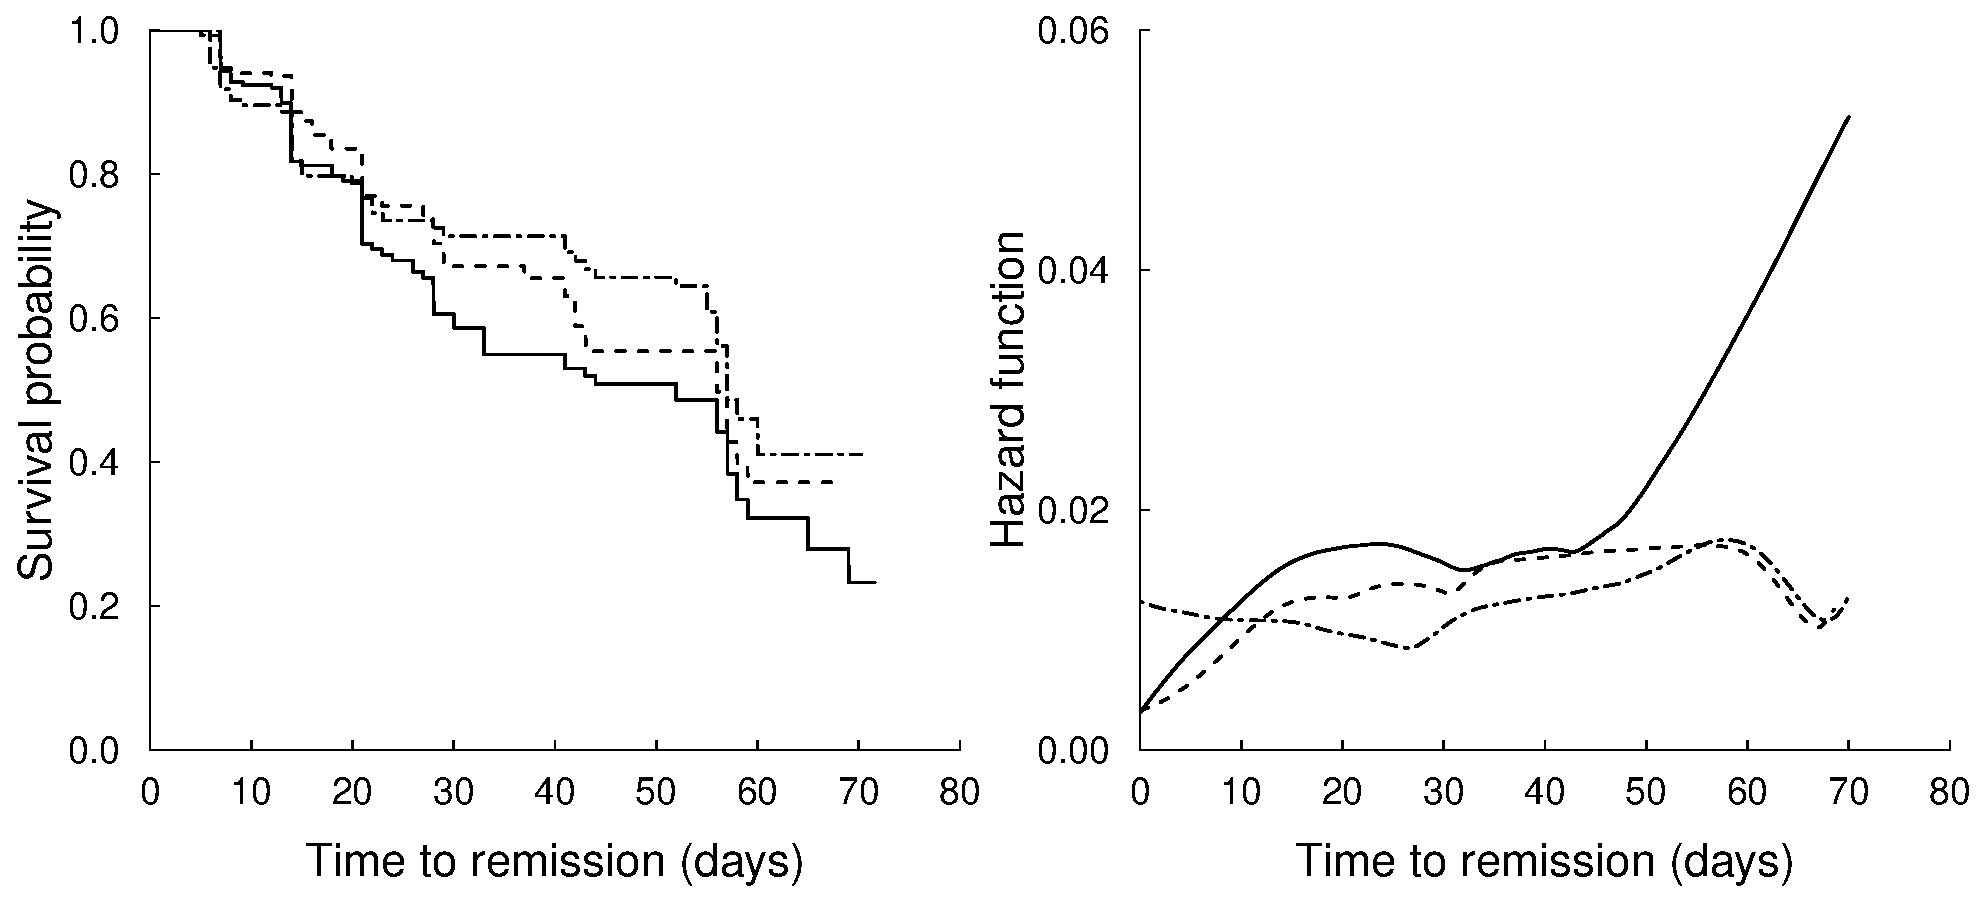
\includegraphics[width=0.99\columnwidth]{figures/paper_survELtest_3arm_surv_haz_20191220.pdf}} %,totalheight=2.0in
	\caption{The KM estimated survival curves (left) and the estimated hazard functions (right) 
		in the \code{threearm} dataset: experimental treatment group (solid), standard treatment group (dashed) and placebo group (two-dashed).
	}
	%\label{fig:Hc}
	\label{fig:threearm}
\end{figure}

%trend test: in page 389/400 of Andersen_book, only log-rank test for trend is mentioned... so let's do it here? (mention PP version if ask)
To see if the curves are statistically significantly ordered, we start with conducting the commonly used log-rank-type tests. The trend test is needed for the one-sided research question. Using the common choice $c(3, 2, 1)$ for the score vector \citep[see, e.g.,][page 388]{Anderson:1993}, the log-rank test for trend is implemented as follows: \\
\begin{example}
>   library(survival)
>   dat = Surv(threearm[, 1], threearm[, 2])
>   logrank = survdiff(dat ~ threearm[, 3])
>   score_vec = 3 : 1
>   logrankteststat = matrix(score_vec, nrow = 1, ncol = 3) 
+   %*% (logrank$obs - logrank$exp) / sqrt(matrix(score_vec, nrow = 1, ncol = 3) 
+   %*% (logrank$var) %*% matrix(score_vec, nrow = 3, ncol = 1))
>   if(logrankteststat < 0){ 
+     pval = 2 * pnorm(logrankteststat)
+   }else{
+     pval = 2 * (1 - pnorm(logrankteststat))
+   }
>   round(pval, 2)

     [,1]
[1,] 0.04
\end{example}
%\code{\quad\quad\quad[,1]} \\
%\code{\quad[1,] 0.04} \\
As the log-rank test for trend gives a $p$-value of $0.04$, we conclude that the three survival functions are ordered at $\alpha=0.05$. 
%brainstorming: trend test no longer the original log-rank formulation; so dangerous to interpret how log-rank arrives at the conclusion the same way as in Sec 3.2 (diff btw j-th group and overall)? but trend test is coxph using score as continuous predictor! so proportional hazards still matter and can be used to interpret why log-rank better than PP in this case!
The other extreme in the $G^\rho$ family can be implemented by setting \code{survdiff(dat {\raise.17ex\hbox{$\scriptstyle\mathtt{\sim}$}} threearm[,~3],~rho = 1)} in the above code, which leads to a $p$-value of $0.08$. These results mean the weighted log-rank statistics in the entire $G^\rho$ family give a $p$-value that ranges from $0.04$ to $0.08$ for the trend test.

Now we conduct the proposed one-sided testing for the \code{threearm} data. We anticipate a more significant result than the log-rank-type tests, as there seems to be crossing among the estimated hazard functions %(i.e., the slopes of the estimated cumulative hazard functions) 
in the right panel of Figure \ref{fig:threearm}, created using the function \code{muhaz} in the package \CRANpkg{muhaz} \cite[][]{muhaz:2019} with the default settings. %, plotted using... (using a similar code in the third paragraph of Section \nameref{sec:use_int}). 
The initial test and the maximally selected EL test are implemented by the routines \code{nocrossings} and \code{supELtest}, respectively. (Note that if two-sided testing is conducted instead, then the initial test is not needed.)
To use the routines, we need to specify two options: \code{sided = 1} for the one-sided test, and \code{group\_order = c(3,~2,~1)}, since the hypothesized order among the three arms with the survival rates ranging from the largest to the smallest is the placebo (coded as 3 in the grouping variable), standard treatment (coded as 2), and experiment treatment (coded as 1). 
The rest of the options are kept at their default values. The R code for performing the initial test is as follows: \\
\begin{example}
>   nocrossings(Surv(threearm$time, threearm$censor) ~ threearm$group, 
+   group_order = c(3, 2, 1), sided = 1)

Call:
nocrossings(formula = Surv(threearm$time, threearm$censor) ~ threearm$group, 
group_order = c(3, 2, 1), sided = 1)

Decision = 1
\end{example}
A decision value of 1 means there is no crossing or alternative orderings among the survival functions. Thus, we can proceed to the main (maximally selected EL) test
in the second step: \\
\begin{example}
>   supELtest(Surv(threearm$time, threearm$censor) ~ threearm$group, 
+   group_order = c(3, 2, 1), sided = 1)

Call:
supELtest(formula = Surv(threearm$time, threearm$censor) ~ threearm$group,
group_order = c(3, 2, 1), sided = 1)

One-sided maximally selected EL test statistic = 14.23, p = 0.004
\end{example}
As the maximally selected EL test gives a $p$-value $<0.01$, we obtain the same conclusion---that the three survival functions are significantly ordered---as the log-rank-type tests for trend, but with a statistically more significant result. This finding is as we anticipated after seeing the crossing estimated hazard functions in the right panel of Figure \ref{fig:threearm}.


%In Figure \ref{fig:threearm}, there is a large local difference appearing at around 50 days. 
Since our procedure leads to the conclusion that the survival functions are ordered, it can be of interest to identify periods of local differences for further clinical investigation. To this end,
%To identify periods of local differences, 
we can use the routine \code{ptwiseELtest} for pointwise testing at each observed uncensored time point:\\
\begin{example}
>   ptwise = ptwiseELtest(Surv(threearm$time, threearm$censor) ~ threearm$group, 
+   group_order = c(3, 2, 1), sided = 1)
\end{example}
The list of the time points at which the survival functions are ordered (i.e., \code{decision == 1}) is obtained by \\ 
\begin{example}
>   round(ptwise$result_dataframe$time_pts[ptwise$result_dataframe$decision == 1], 2)

 [1] 13.91 13.91 13.91 13.92 13.92 13.92 13.92 13.93 13.98 13.99 13.99 14.00 14.00
[14] 14.00 14.01 14.01 20.96 20.96 27.98 27.99 28.00 28.00 28.00 28.02 28.02 28.98
[27] 28.99 29.01 30.00 32.96 36.97 40.97 40.98 40.99 41.02 41.98 41.98 41.99 42.00
[40] 42.01 42.02 42.99 43.01 43.02 43.02 44.00 44.00 51.97 51.97 55.00 56.01 56.01
[53] 56.02 59.03 59.04 64.97 68.98 69.01
\end{example}
From the result, we see there are local differences occurring near the time points 14, 21, 30, 40, 52, 56, 59, 65 and 69 days. %This confirms the differences can also be observed from the left panel of Figure \ref{fig:threearm}
%To detect such a difference, Kolmogorov--Smirnov-type statistics like Kn can be used.
%This information can be used for designing further study.


\subsection{Application of intELtest to hepatitis data}\label{sec:use_int}
%just put in what you want your friends know first

Now we turn to our motivating example in the Introduction and
demonstrate the use of \code{intELtest} and its benefit over the log-rank-type tests. The corresponding dataset \code{hepatitis} is provided in the \pkg{survELtest} package.  %The data come from digitizing the published KM curves in \citet{hepatitis:2011} and reconstructing survival and censoring information using the algorithm developed by \citet{KMreconstruct:2012}. 
The dataset was obtained by reconstructing survival and censoring information \citep[][]{KMreconstruct:2012} based on digitizing the KM curves presented in  \citet{hepatitis:2011}. It contains survival data (in days, rounded to one decimal place) from patients in a randomized clinical trial for the treatment of severe alcoholic hepatitis.
The purpose of the clinical trial was to assess if the treatment group ($n_1=85$) had a significantly different survival rate than the control group ($n_2=89$). %While this question is a one-sided hypothesis, %since two-sided tests are usually considered in clinical trials, 
%since the original paper used the two-sided log-rank test, we will demonstrate results of both two-sided and one-sided testing.


From the KM estimated survival curves in Figure \ref{fig:hepatitis}, 
the survival rate of the treatment group seems to be greater than that of the control group over the entire follow-up period. To see whether the difference between the survival functions are statistically significant, %we conduct formal hypothesis testing. 
%W
we start with conducting the commonly used two-sided log-rank test: \\ 
\begin{example}
>   library(survival)
>   dat = Surv(hepatitis[, 1], hepatitis[, 2])
>   logrank = survdiff(dat ~ hepatitis[, 3])
>   round(1 - pchisq(logrank$chisq, df = 1), 2)

[1] 0.07
\end{example}
\noindent The log-rank test gives a $p$-value of $0.07$, failing to detect a difference between the survival curves at $\alpha=0.05$. The reason may be due to the crossing estimated hazard functions in Figure \ref{fig:hepatitis_haz} (created using the function \code{muhaz} in the package \pkg{muhaz} with the default settings).
%From Figure \ref{fig:hepatitis_haz}, the estimated hazard functions (that is, the slopes of the two curves) seem to cross at around day 60. %As the log-rank statistic sums up differences between the two estimated hazard functions over the follow-up period, t
%The crossing means the cumulative differences after day 60 would cancel out with that before day 60 due to their opposite signs.
%differ noticeably only during the initial 40 days, but remain similar afterwards. %, as can be seen by comparing the slopes of cumulative hazards functions. 
%This means only the initial follow-up period is contributing to any difference that the log-rank test is detecting, and
%This may be why the log-rank statistic is not large enough to conclude a significant difference between the two groups at $\alpha=0.05$.
We also conduct another log-rank-type test---the Peto and Peto's modification of the Gehan-Wilcoxon test---by setting \code{survdiff(dat {\raise.17ex\hbox{$\scriptstyle\mathtt{\sim}$}} hepatitis[,~3],~rho = 1)} in the above code, which leads to a $p$-value of $0.05$. 
Since this test and the log-rank test are the two extremes in the $G^\rho$ family, these results mean the weighted log-rank statistics in the entire $G^\rho$ family give either insignificant or borderline significant conclusions. 
%note that varying rho... but it is hard to know a priori which test gives the most significant result... (then mention thi sin beginning of the section)


\begin{figure}[H] %width = 0.5
	\centerline{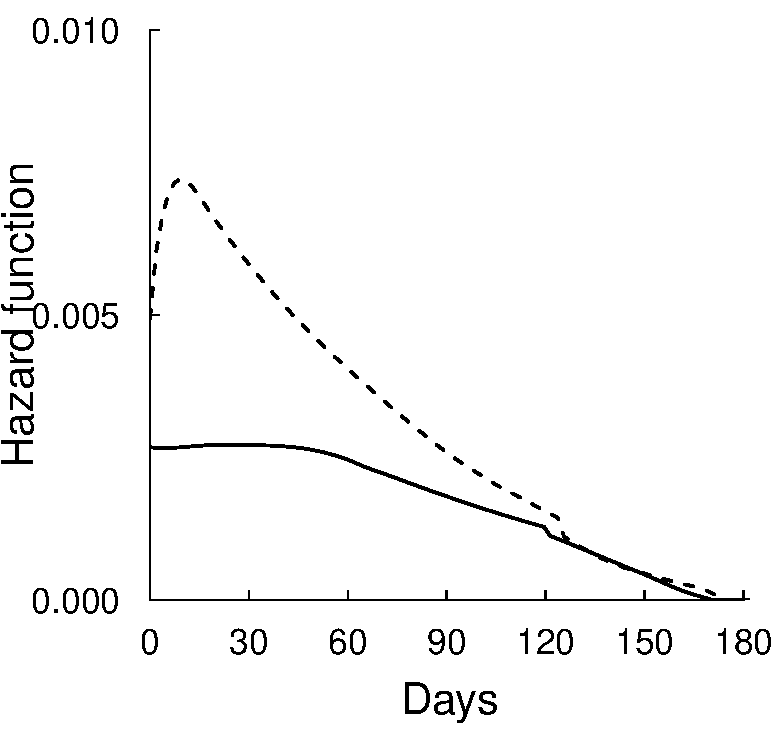
\includegraphics[width=0.5\columnwidth]{figures/paper_survELtest_hep_haz_20191220.pdf}} %,totalheight=2.0in
	\caption{Estimated hazard functions
		for treatment (solid line) versus control (dashed line) groups.
	}
	\label{fig:hepatitis_haz}
\end{figure}
\noindent 

% They concluded that the combination therapy does not improve the 6-month survival. In contrast, our two-sided EL test shows that the two treatment groups are significantly different and there is a uniformly higher survival function in one of the groups ($p=0.036$, computed by the supplementary {\tt R} program that implements the two-sided EL test). In this case the EL test shows a more significant result that leads to a completely different conclusion than the log-rank test.


Now we apply the proposed two-sided integrated EL test
to the \code{hepatitis} data to see if we can better detect a difference between the survival functions. 
The default options are used and 
the R code is as simple as \\
\begin{example}
>   intELtest(Surv(hepatitis$time, hepatitis$censor) ~ hepatitis$group)

Call:
intELtest(formula = Surv(hepatitis$time, hepatitis$censor) ~ hepatitis$group)

Two-sided integrated EL test statistic = 1.42, p = 0.007
\end{example}
As the integrated EL test gives a $p$-value $<0.01$, we conclude there is a significant difference between the two survival functions at $\alpha=0.05$. The $p$-value is much smaller than those given by the previous log-rank-type tests, %The same conclusion can be drawn from the fact that the test statistic $1.41$ is greater than the critical value $0.90$. 
which indicates that the integrated EL test is better at detecting the difference between the survival curves.

Note the decision as to whether there is a significant discrepancy between the two survival functions is totally different for the log-rank and the integrated EL tests at $\alpha=0.05$. It may be tempting to pick the most significant result, but this practice is data snooping and has been shown to be problematic. 
Instead, we recommend setting a primary method prior to the data analysis and making the decision based on that method. Any other methods are treated as secondary, and their results can serve an exploratory purpose for future work. 


\section{Discussion}\label{sec:discussion}

In this paper we introduce the R package \pkg{survELtest} for comparing two or more survival functions nonparametrically based on right-censored data. It is the only R package to date that utilizes the powerful likelihood ratio formulation instead of log-rank-type statistics, thereby performing well when the hazard functions cross.
%does not use log-rank-type statistics for the task, thereby avoiding the pitfall of the log-rank-type formulation when the hazard functions cross.
%in which negative and positive differences between the estimated hazard functions cancel with each other in a weighted sum
We provide both maximal-deviation-type and integral-type statistics, for detecting local and cumulative differences among the survival functions, respectively.

The use of the software is illustrated using two data sets from randomized clinical trials, where the estimated survival functions seem to be ordered, but the estimated hazard functions cross. In these cases, our procedures lead to more significant results than the results obtained from the log-rank-type tests. Specifically, in one of the examples, the original clinical trial concludes that there is no significant difference between the treatment and the control groups (log-rank $p=0.07$), whereas our test suggests otherwise, based on a much smaller $p$-value $<0.01$.
%gives $p=0.01$, a much smaller $p$-value.
%Other scenarios when the estimated hazard functions do not cross have also been investigated \citep{CM:2016, CM:2019}, where our methods are shown to compete effectively with the log-rank test.
We envision the \pkg{survELtest} package will be valuable for finding more significant results in numerous biomedical settings involving the comparison of multiple survival functions, especially in the presence of crossing hazards.



\bigskip

\section{Availability} \label{sec:avail}

The package is available from the Comprehensive R
Archive Network at \url{https://CRAN.R-project.org/package=survELtest}.
The development website is available at \url{https://github.com/news11/survELtest}.



\section{Acknowledgements}  The research of Hsin-wen Chang was partially supported by Ministry of Science and Technology of Taiwan under grants 106-2118-M-001-015-MY3 and MOST 109-2118-M-001-005-. The authors thank Yu-Ju Wang for computational support and Shih-Hao Huang for helpful comments. The authors declare that they have no conflict of interest.

\bibliography{chang} 

\address{Hsin-wen Chang\\
Institute of Statistical Science\\
Academia Sinica\\
128 Academia Road, Section 2,\\
Nankang, Taipei 11529, Taiwan (R.O.C)\\
ORCiD: 0000-0003-4566-7047\\
\email{hwchang@stat.sinica.edu.tw}
}

\address{Pei-Yuan Tsai\\
Institute of Statistical Science\\
Academia Sinica\\
Taipei, Taiwan (R.O.C)
}

\address{Jen-Tse Kao\\
Institute of Statistical Science\\
Academia Sinica\\
Taipei, Taiwan (R.O.C)
}

\address{Guo-You Lan\\
Department of Economics\\
National Chengchi University\\
Taipei, Taiwan (R.O.C)
}

\newpage
	
%% The Appendices part is started with the command \appendix;
%% appendix sections are then done as normal sections
\appendix

\section{Appendix: Comparison of \pkg{survELtest} with other existing tests in two simulated datasets} \label{app:2egs}

Here we provide two more examples for comparing our procedures with other existing tests in the literature, namely the log-rank test, the Peto and Peto's modification of the Gehan-Wilcoxon test, the adaptive weighted log-rank test implemented in  the R  package \pkg{YPmodel}, and the RMST method implemented in  the R  package \pkg{survRM2}.
Since the latter two methods cannot deal with the general $k$-sample case nonparametrically, the examples provided here are restricted to the two-sample case.
For the first dataset \code{hazardcross}, the survival time is generated from the piecewise exponential model displayed in the left panel of Figure \ref{fig:2egs}. %1 in \citet{CM:2016}. 
Since the difference between the true survival curves appears only during $[0, 6]$ but not later on, we use \code{supELtest} to detect such local differences.
For the second dataset \code{hazardcross\_Weibull}, the survival time is generated from the Weibull model displayed %as the solid and dashed lines
in the right panel of Figure \ref{fig:2egs}. %1 in \citet{CM:2019}. 
We use \code{intELtest} because the difference between the true survival curves is spread over the entire follow-up period.
For both datasets, the true hazard functions cross, but there is an obvious gap between the survival curves.
The censoring distributions are specified to be the same in each arm, and uniform with administrative censoring at t = 10 and a censoring rate of 25\% in the first group. We use the default settings in implementing the tests given in
the aforementioned two packages.

The results are given in Table \ref{table:2egs}. Our tests provide more significant results in detecting the gap between the survival curves than any of the other tests for both datasets.
 
 \begin{figure}[H]
 	\centerline{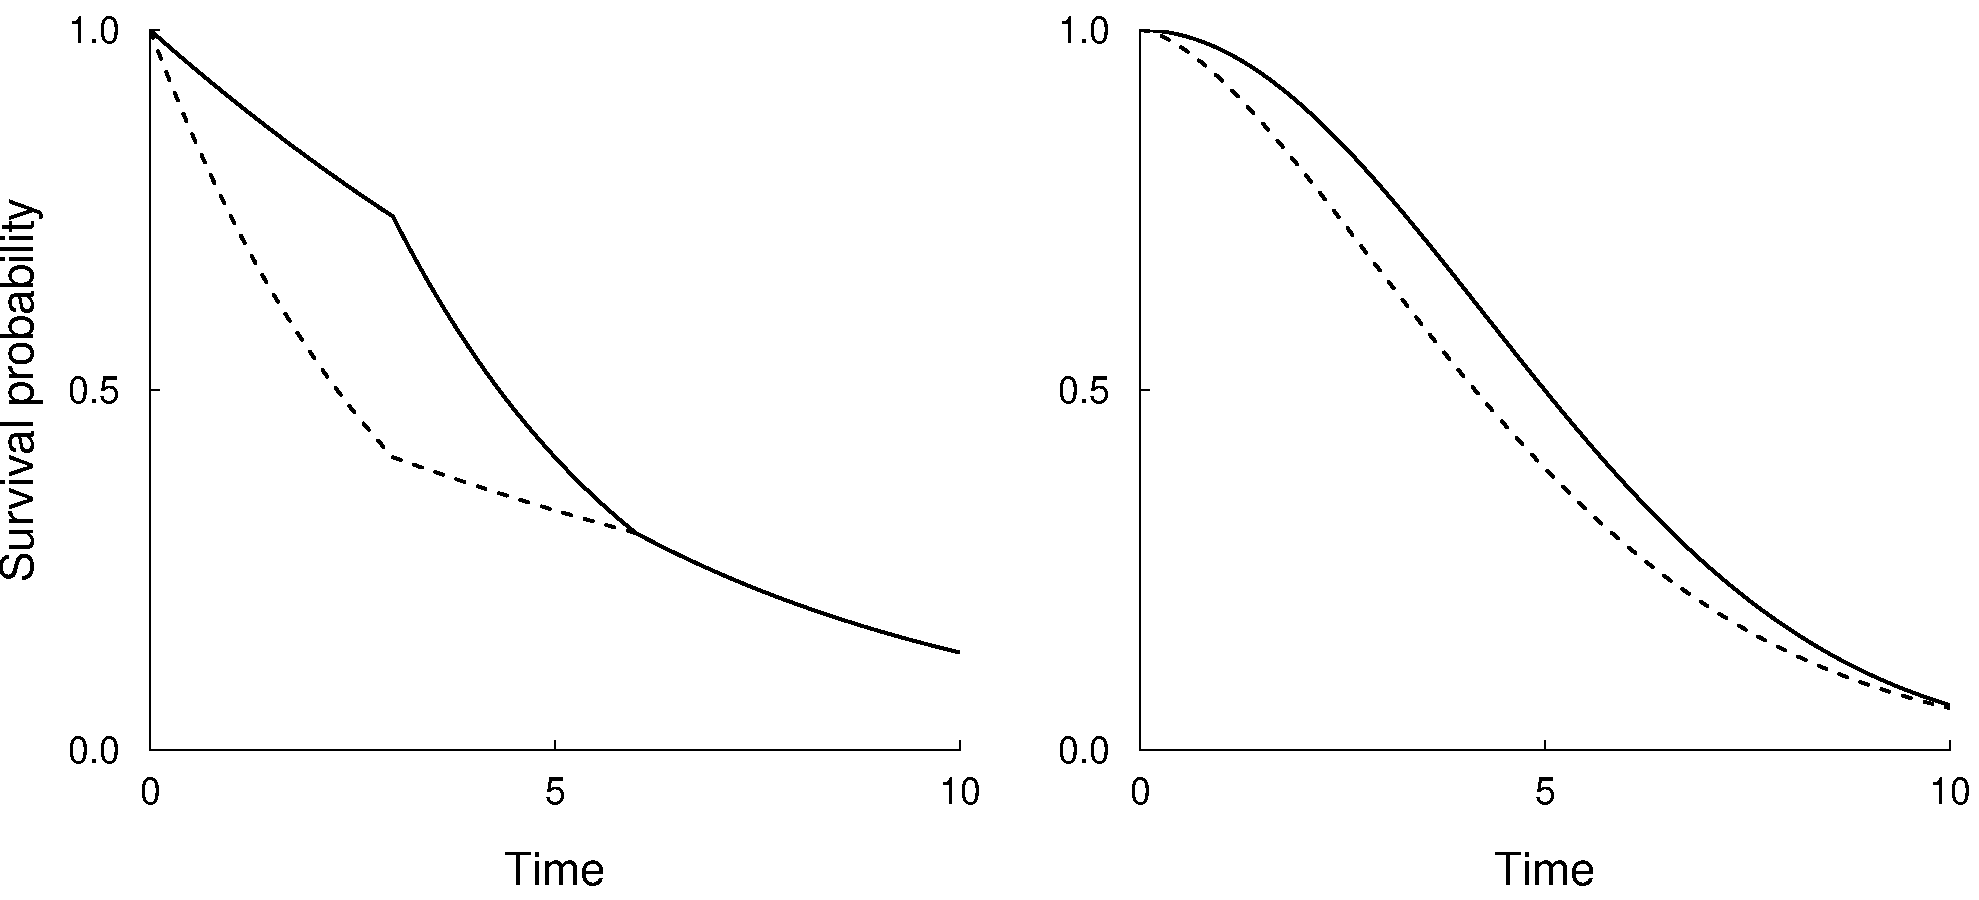
\includegraphics[width=0.99\columnwidth]{figures/paper_EL2Surv_2egs.pdf}} %,totalheight=2.0in
 	\caption{
 	The true survival curves for generating \code{hazardcross} (left) and  \code{hazardcross\_Weibull} (right) datasets: the first (solid) and second (dashed) groups.
 	}
 	%\label{fig:Hc}
 	\label{fig:2egs}
 \end{figure}
 
 \begin{table}[h!] 
  	\centering
   \caption{$p$-values from various tests for comparing the survival curves in the \code{hazardcross} and  \code{hazardcross\_Weibull} datasets. EL denotes the suitable EL test implemented in the R package \pkg{survELtest},	PP denotes the Peto and Peto's modification of the Gehan-Wilcoxon test, YP denotes the adaptive weighted log-rank test implemented in  the R  package \pkg{YPmodel}, and dRMST and rRMST denote the results in  the R  package \pkg{survRM2} for the difference in and the ratio of RMST, respectively. 
   }
 \medskip
  	\label{table:2egs}
  	\begin{tabular*}{\columnwidth}{@{}l@{\extracolsep{\fill}}r@{\extracolsep{\fill}}r@{\extracolsep{\fill}}r@{\extracolsep{\fill}}r@{\extracolsep{\fill}}r@{\extracolsep{\fill}}r@{\extracolsep{\fill}}@{}} \toprule
 	\centering
     %\multirow{2}{*}{} & \multicolumn{2}{c}{$[\alpha_1, \alpha_2]$} & \multicolumn{3}{c}{$[0.05,0.95]$}&  \multicolumn{3}{c}{$[0.1,0.9]$}\\ \cline{2-3} \cline{4-6} \cline{7-9}
     %& 
     Datasets & EL & log-rank & PP & YP & dRMST & rRMST \\ \midrule %\hline
 	%\multirow{4}{*}{Coverage (Average Width)}  &   
 	\code{hazardcross} & 0.037 & 0.106 & 0.060 & 0.096 & 0.126 & 0.130 \\ %\cline{1-10} % 20190111 all groups done
 	
     %&  
     \code{hazardcross\_Weibull} & 0.005 & 0.080 & 0.006 & 0.009 & 0.014 & 0.018 \\   \bottomrule % 20190111 done
  	\end{tabular*} %\vskip18pt
  \end{table} 
 

